%!TEX options = -shell-escape

\documentclass[12pt]{report}
\usepackage[a4paper,twoside,top=20mm,bottom=20mm,inner=30mm,outer=25mm]{geometry}
\usepackage[utf8]{inputenc}
\usepackage[greek,english]{babel}
\usepackage[scaled=0.86]{couriers}
\usepackage[toc,page,title,titletoc]{appendix}
\usepackage[pdfpagelabels,unicode]{hyperref}
\usepackage{bookmark}
\usepackage[fixlanguage]{babelbib}
\selectbiblanguage{greek}
\usepackage{titlesec}
\usepackage{etoolbox}
\usepackage{graphicx}
\usepackage{array}
\usepackage{amsmath}
\usepackage{minted}
\usepackage{subcaption}
\captionsetup{compatibility=false}
\graphicspath{ {images/} }
\usepackage[noend]{algpseudocode}
\usepackage{algorithm}
\usepackage{afterpage}
\usepackage{comment}

\newcommand\blankpage{%
    \null
    \thispagestyle{empty}%
    \addtocounter{page}{-1}%
    \newpage}

\hypersetup{
  colorlinks=true,
  % linkcolor=green,
  citecolor=red,
  % filecolor=blue,
  urlcolor=blue,
  % pdftitle=,
  % pdfauthor=,
  % pdfsubject=,
  % pdfkeywords=
}

\setcounter{secnumdepth}{3}
\setcounter{tocdepth}{3}

\titleformat{\chapter}
  {\normalfont\LARGE\bfseries}{\thechapter}{1em}{}
\titlespacing*{\chapter}{0pt}{3.5ex plus 1ex minus .2ex}{2.3ex plus .2ex}

\makeatletter
\patchcmd\@resets@pp{%
  \def\Hy@chapapp{\appendixname }%
}{%
  \def\Hy@chapapp{appendix}%
}{}{\errmessage{Cannot patch \string\@resets@pp}}
\patchcmd\@resets@ppsub{%
  \def\Hy@chapapp{\appendixname }%
}{%
  \def\Hy@chapapp{appendix}%
}{}{\errmessage{Cannot patch \string\@resets@pp}}
\makeatother

\addto{\captionsgreek}{\renewcommand{\appendixpagename}{Παραρτήματα}}
\addto{\captionsgreek}{\renewcommand{\appendixtocname}{Παραρτήματα}}
\addto{\captionsgreek}{\renewcommand{\appendixname}{Παράρτημα}}

\begin{document}
\selectlanguage{greek}

\hypersetup{pageanchor=false}

\begin{titlepage}
  \centering
  
\includegraphics[width=0.15\textwidth]{pyrforos}\par\vspace{1cm}
  {\scshape\LARGE Εθνικό Μετσόβιο Πολυτεχνείο\\
  Σχολή Ηλεκτρολόγων Μηχανικών και Μηχανικών Η/Υ\par}
  \vspace{1cm}
  {\scshape\Large Εργασία στο Μεταπτυχιακό Μάθημα\\
  Διαχείριση Τεχνολογιών στο Ηλεκτρονικό Εμπόριο\par}
  \vspace{1.5cm}
  {\Large\bfseries Ανάπτυξη Ιστοσελίδας Ηλεκτρονικών Δημοπρασιών\par}
  \vspace{2cm}
  {\large Δημήτριος Πολίτης (ΥΔ)\par}
  \vfill
  Επιβλέπων \par
  Καθ. Ευστάθιος Συκάς

  \vfill

% Bottom of the page
  {\large \today\par}
  \afterpage{\blankpage}
\end{titlepage}

\tableofcontents
\thispagestyle{empty}

\listoftables
\thispagestyle{empty}

\listoffigures
\thispagestyle{empty}

\begin{abstract}
Στο παρόν παρουσιάζεται η λειτουργία και η διαδικασία ανάπτυξης μιας ιστοσελίδας δημοπρασιών. Αρχικά  γίνεται αναφορά στις βασικές έννοιες του ηλεκτρονικού εμπορίου Παρουσιάζονται αρχικά τα διαθέσιμα λογισμικά, τα πλεονεκτήματα και μειονεκτήματά τους και στη συνέχεια περιγράφεται αναλυτικά η διαδικασία δημιουργίας ενός ιστοτόπου ηλεκτρονικών δημοπρασιών με τη χρήση αυτοματοποιημένων εργαλείων (\textlatin{phpProBid, vagrant}).

\vspace{10mm}

\noindent \textbf{Λέξεις κλειδιά:} Ηλεκτρονικό Εμπόριο, Ηλεκτρονική Δημοπρασία, Ανοιχτός Κώδικας, Εξυπηρετητής Ιστοσελίδων, Διαδίκτυο.
\end{abstract}

\hypersetup{pageanchor=true}
\clearpage
\pagenumbering{arabic}

\chapter{Εισαγωγή}\label{ch1}
\section{Εισαγωγή}
Η εποχή του διαδικτύου επιβάλει την αναθεώρηση των παραδοσιακών τρόπων διεξαγωγής του εμπορίου, μέσω φυσικής επαφής. Πλέον μεγάλο ποσοστό των εμπορικών συναλλαγών, τόσο μεταξύ επιχειρήσεων, όσο και μεταξύ ιδιωτών και επιχειρήσεων, πραγματοποιούνται με ηλεκτρονικά μέσα.

Η δημιουργία, η συντήρηση και η ανανέωση του περιεχομένου των ιστοτόπων ηλεκτρονικών αγορών αποτελεί μοχλό μεγέθυνσης των πωλήσεων και σε βάθος χρόνου, του κύκλου εργασιών.

\section{Ηλεκτρονικό Εμπόριο}
\subsection{Ορισμοί - Έννοιες}
Το Ηλεκτρονικό Εμπόριο (ΗΕ) περιγράφει τη διαδικασία αγοράς, πώλησης, μεταφοράς ή ανταλλαγής προϊόντων , υπηρεσιών ή/και πληροφοριών μέσω δικτύων υπολογιστών, περιλαμβανομένου και του Διαδικτύου~\cite{turban_outland_king_lee_liang_turban_2018}. Το ΗΕ μπορεί να οριστεί από τις παρακάτω σκοπιές:
  \paragraph{Επιχειρησιακή Διεργασία.} Από την σκοπιά των επιχειρησιακών διεργασιών το ΗΕ αφορά στην εκτέλεση των διεργασιών με ηλεκτρονικό τρόπο, ολοκληρώνοντας ηλεκτρονικές διεργασίες μέσω δικτύων Η/Υ.
  \paragraph{Εξυπηρέτηση.} Από τη σκοπιά των επιχειρήσεων, το ΗΕ είναι ένα εργαλείο που απευθύνεται στη επιθυμία των κυβερνήσεων, των εταιριών, των πελατών και της διοίκησης να περικόψουν το κόστος των υπηρεσιών ενώ ταυτόχρονα να βελτιώσουν την παρεχόμενη ποιότητα των υπηρεσιών και ταχύτητα εξυπηρέτησης.
  \paragraph{Εκπαίδευση.} Από τη σκοπιά της εκπαίδευσης, το ΗΕ παρέχει την δυνατότητα εκπαίδευσης και επιμόρφωσης \textlatin{online} σε σχολεία, πανεπιστήμια και επιχειρήσεις.
  \paragraph{Συνεργατική.} Από τη σκοπιά της συνεργασίας είναι το πλαίσιο της ενδοεπιχειρησιακής και διαεπιχειρησιακής συνέχειας.
  \paragraph{Κοινωνική.} Από την κοινωνική σκοπιά, το ΗΕ παρέχει μια θέση συγκέντρωσης μελών της κοινωνίας για εκμάθηση, συνδιαλλαγή και συνεργασία.

Πολλές φορές το ΗΕ συγχέεται με το Ηλεκτρονικό Επιχειρείν, μια πιο ευρεία έννοια. Το Ηλεκτρονικό Επιχειρείν αναφέρεται στον ευρύτερο ορισμό του ΗΕ, όχι μόνο στην αγορά και την πώληση των αγαθών αλλά και επίσης στην εξυπηρέτηση πελατών, στη συνεργασία με επιχειρηματικούς εταίρους, στη διεξαγωγή ηλεκτρονικής εκπαίδευσης και την διεξαγωγή ηλεκτρονικών συναλλαγών εντός των ορίων του οργανισμού.

Σύμφωνα με το~\cite{chen_2005} το Ηλεκτρονικό Επιχειρείν είναι η χρήση του Διαδικτύου και άλλων τεχνολογιών της πληροφορικής για την υποστήριξη του εμπορίου και τη βελτίωση της απόδοσης μιας επιχείρησης.

\subsection{Αμιγές και Μερικό ΗΕ}
Το ηλεκτρονικό εμπόριο μπορεί να πάρει πολλές μορφές ανάλογα με το βαθμό ψηφιοποίησης των παρακάτω παραγόντων:
\begin{itemize}
  \item του προϊόντος - υπηρεσίας προς πώληση
  \item της διαδικασίας (για παράδειγμα παραγγελία ή πληρωμή)
  \item της μεθόδου διανομής
\end{itemize}

Στο~\cite{choi_stahl_whinston_1997} παρουσιάζεται ένα μοντέλο που περιγράφει τους πιθανούς συνδυασμούς αυτών των τριών διαστάσεων. Ένα προϊόν μπορεί να είναι φυσικό ή ψηφιακό, η μέθοδος διανομής μπορεί να είναι φυσική η ηλεκτρονική, Η διαδικασία μπορεί αναλόγως να είναι φυσική η ψηφιακή. Η περιγραφή αυτή γίνεται κατανοητή εφόσον παρατηρήσουμε το~\ref{fig:ec_dimensions}.
\begin{figure}[h]
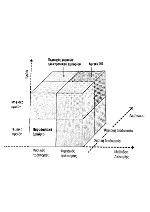
\includegraphics[width=0.9\linewidth, height=7cm]{ec-dimensions}
\caption{Μέθοδος Αποδοχής - Απόρριψης}
\label{fig:ec_dimensions}
\end{figure}
\subsection{Μειονεκτήματα}



\section{Συμπεράσματα}
Στο παρόν, παρουσιάστηκε ένα μοντέλο προσομοίωσης του πρωτοκόλλου πολλαπλής πρόσβασης μέσου (\textlatin{MAC}) τύπου \textlatin{slotted aloha}. Τα αποτελέσματα της προσομοίωσης έδειξαν τιμές πολύ κοντά στις θεωρητικά αναμενόμενες. Συγκεκριμένα, η αύξηση των μνημών προσωρινής αποθήκευσης πακέτων (\textlatin{receiving buffers}) στους σταθμούς, είχε θετική επίδραση στην απόδοση του συστήματος \textlatin{S}, η οποία όμως εμφανίζονταν φθίνουσα, καθώς αυξάνονταν το πλήθος των σταθμών \textlatin{M}. Επίσης, η αύξηση του πλήθους των \textlatin{receiving buffers} πάνω από δύο, δεν είχε κάποια σημαντική επίδραση στην αποδοτικότητα του συστήματος. Αντιθέτως, η αύξηση των διαύλων επικοινωνίας μεταξύ των κόμβων είχε σημαντικά θετική επίδραση στην διεκπεραιωτική δυνατότητα του συστήματος και τη μείωση της καθυστέρησης, ανεξάρτητα από το πλήθος των σταθμών.

Τα παραπάνω καταδεικνύουν ότι η βέλτιστη απόδοση του πρωτοκόλλου επιτυγχάνεται όταν οι σταθμοί έχουν δύο το πλήθος \textlatin{receiving buffers} και ικανό αριθμό καναλιών - διαύλων επικοινωνίας μεταξύ τους (ο οποίος μπορεί να περιορίζεται από τεχνικούς περιορισμούς ή περιορισμούς κόστους). Στην περίπτωση των ασύρματων δικτύων αυτό μπορεί να μεταφραστεί: είτε σε ικανό αριθμό πομποδεκτών ανά σταθμό, οι οποίοι θα λειτουργούν σε διαφορετικές συχνότητες για λόγους αποφυγής παρεμβολών, είτε σε κατάλληλο σχήμα πολύπλεξης (\textlatin{TDM, FDM}), επαναχρησιμοποίηση φάσματος με αναπήδηση συχνότητας κ.α. Κατά αντιστοιχία, στα οπτικά δίκτυα είναι δυνατή η χρησιμοποίηση πολύτροπων οπτικών ινών και εκπομπή των δεδομένων σε διαφορετικά μήκη κύματος για την ταυτόχρονη χρησιμοποίηση του μέσου.

\begin{appendices}

\end{appendices}

\appendix

\bibliographystyle{babplain}
\bibliography{e-commerce}

\end{document}